\tikzstyle{box} = [rectangle, minimum width=3cm, minimum height=1cm, text centered, draw=black]
\tikzstyle{arrow} = [thick,->,>=stealth]

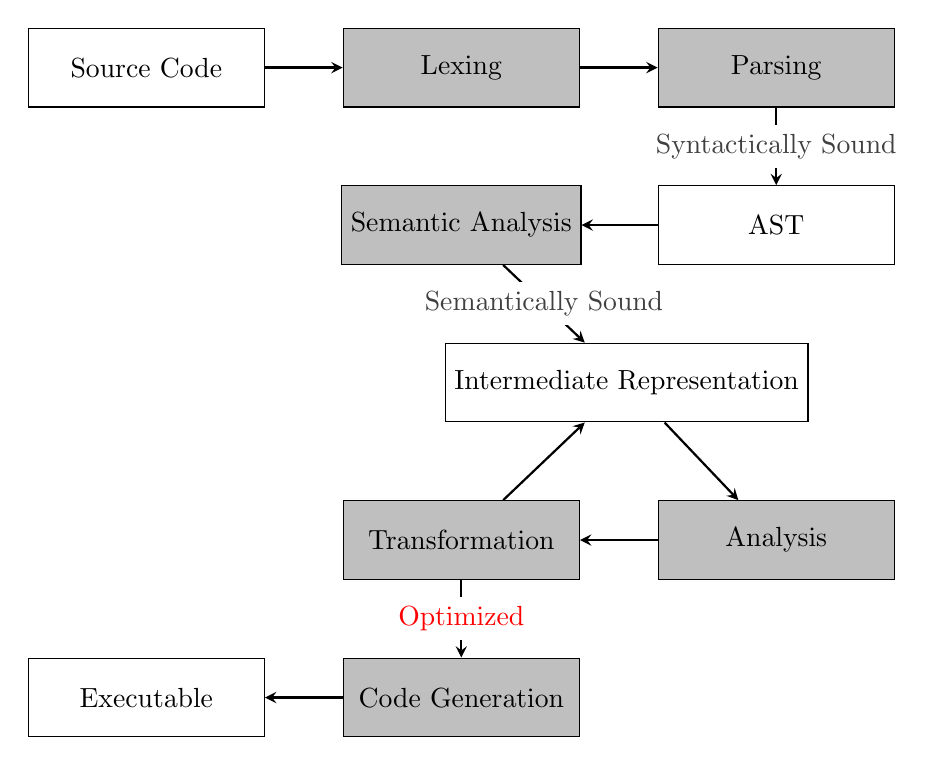
\begin{tikzpicture}
  \node (Source Code) [box] {Source Code};
  \node (Lexing) [box, fill=lightgray, right of=Source Code, xshift=3cm] {Lexing};
  \node (Parsing) [box, fill=lightgray, right of=Lexing, xshift=3cm] {Parsing};
  \node (AST) [box, below of = Parsing, yshift=-1cm] {AST};
  \node (Semantic Analysis) [box, fill=lightgray, left of=AST, xshift=-3cm] {Semantic Analysis};
  \node (Intermediate Representation) [box, below of=Semantic Analysis, yshift=-1cm, xshift=2.1cm] {Intermediate Representation};
  \node (Analysis) [box, fill=lightgray, below of=Intermediate Representation, yshift=-1cm, xshift=1.9cm] {Analysis};
  \node (Transformation) [box, fill=lightgray, left of=Analysis, xshift=-3cm] {Transformation};
  \node (Code Generation) [box, fill=lightgray, below of=Transformation, yshift=-1cm] {Code Generation};
  \node (Executable) [box, left of=Code Generation, xshift=-3cm] {Executable};

  \draw [arrow] (Source Code) -- (Lexing);
  \draw [arrow] (Lexing) -- (Parsing);
  \draw [arrow] (Parsing) -- node [fill=white, text=darkgray] {Syntactically Sound} (AST);
  \draw [arrow] (AST) -- (Semantic Analysis);
  \draw [arrow] (Semantic Analysis) -- node [fill=white, text=darkgray] {Semantically Sound} (Intermediate Representation);
  \draw [arrow] (Intermediate Representation) -- (Analysis);
  \draw [arrow] (Analysis) -- (Transformation);
  \draw [arrow] (Transformation) -- (Intermediate Representation);
  \draw [arrow] (Transformation) -- node [fill=white, text=red] {Optimized} (Code Generation);
  \draw [arrow] (Code Generation) -- (Executable);
\end{tikzpicture}